%% packages
\documentclass{article}
\usepackage[a4paper, left=1.5cm, right=1.5cm, top=3.5cm]{geometry}
\usepackage[ngerman]{babel}
\usepackage{graphicx}
\usepackage{multicol}
\usepackage{amssymb}
\usepackage{titlesec}
\usepackage{wrapfig}
\usepackage{blindtext}
\usepackage{lipsum}
\usepackage{caption}
\usepackage{listings}
\usepackage{fancyhdr}
\usepackage{nopageno}
\usepackage{authblk}
\usepackage{amsmath} % tons of math stuff
\usepackage{mathtools} % e.g. alignment within matrix
%\usepackage{bm} % provides shorthand for bold in math mode
\usepackage{dsfont} % \mathds makes double stroke digits
\usepackage{esdiff} % provides \diff
%\usepackage[ISO]{diffcoeff}
\usepackage{xcolor}
\usepackage{csquotes} % e.g. provides \enquote
\usepackage{siunitx} % units
\usepackage{xcolor} % colored text
%\fancyhf[]{}


%% custom stuff
% own units
\DeclareSIUnit \VSS {\ensuremath{V_\mathrm{SS}}}
\DeclareSIUnit \VS {\ensuremath{V_\mathrm{S}}}
\DeclareSIUnit \Veff {\ensuremath{V_\mathrm{eff}}}
\DeclareSIUnit \Vpp {\ensuremath{V_\mathrm{pp}}}
\DeclareSIUnit \Vp {\ensuremath{V_\mathrm{p}}}
\DeclareSIUnit \VRMS {\ensuremath{V_\mathrm{RMS}}}
\DeclareSIUnit \ASS {\ensuremath{A_\mathrm{SS}}}
\DeclareSIUnit \AS {\ensuremath{A_\mathrm{S}}}
\DeclareSIUnit \Aeff {\ensuremath{A_\mathrm{eff}}}
\DeclareSIUnit \App {\ensuremath{A_\mathrm{pp}}}
\DeclareSIUnit \Ap {\ensuremath{A_\mathrm{p}}}
\DeclareSIUnit \ARMS {\ensuremath{A_\mathrm{RMS}}}

% change subsection numbering to capital letters
\newcommand{\subsectionAlph}{ \renewcommand{\thesubsection}{\arabic{section}.\Alph{subsection}} }
% change subsection numbering to lowercase letters
\newcommand{\subsectionalph}{ \renewcommand{\thesubsection}{\arabic{section}.\alph{subsection}} }
% own fig. that works with multicols
\newenvironment{Figure}
  {\par\medskip\noindent\minipage{\linewidth}}
  {\endminipage\par\medskip}
\newcommand*{\inputPath}{./plot} % prepend this command to the argument of all input commands
\graphicspath{ {./figure/} }


% own commands
% \newcommand{\rarr}{$\to\,$} %A$\,\to\,$B
\newcommand{\defc}{black}
\newcommand{\colorT}[2][blue]{\color{#1}{#2}\color{\defc}}
\newcommand{\redq}{\color{red}(?)\color{\defc}}
\newcommand{\question}[1]{\colorT[purple]{\textbf{(#1)}}}
\newcommand{\todo}[1]{\colorT[red]{\textbf{(#1)}}}
\newcommand{\mr}{\mathrm}

%% preparation
\begin{titlepage}
    \title{Elektronikpraktikum: Versuch 1 \\Ausbreitung von Signalen auf Leitungen}
    \author[1]{Marc Hauer\thanks{s??mhaue@uni-bonn.de}}
    \author[1]{Michael Vogt\thanks{s65mvogt@uni-bonn.de}}
    \affil[1]{Uni Bonn}
    %\date{\today}
\end{titlepage}


%% document
\begin{document}

\pagenumbering{gobble}
\maketitle
\tableofcontents
\newpage
\pagenumbering{arabic}

\pagestyle{fancy}
\fancyhead[R]{\thepage}
\fancyhead[L]{\leftmark}

\todo{Allgemeine Fragen beantworten können!}
Es sollen die Eigenschaften von Koaxialkabeln und die wellenartige Ausbreitung von Signalen durch diese Leiter untersucht werden.

\section{Theorie}
Ein Koaxkabel besteht aus einem inneren Leiter, der durch ein Dielektrikum von einem äußeren, zylinderförmigen Leiter getrennt ist.
Der äußere Leiter dient als Erdelektrode und/oder zur Abschirmung äußerer Felder. Durch diesen Aufbau hat das Kabel sowohl eine
Kapazität $C$, als auch eine Induktivität $I$, welche die Signalausbreitung maßgeblich beeinflussen \todo{+Formeln für C und I}.
Hinzu kommen die charakteristischen Größen Verlustleitwert (\enquote{Ableitung}) $G$ und Widerstand $R$,
welche den Verlustwiderstand parallel zur Kapazität bzw. in Reihe zur Induktivität beschreiben.
All diese Größen wachsen linear mit der Länge des Kabels. Daher werden Längenunabhängige Größen eingeführt,
bei denen ein Hochkomma an das Formelzeichen gesetzt wird, z.B. $R' = R/l$ mit der Leiterlänge $l$.

Zur Veranschaulichung kann das Kabel als Reihenschaltung vieler kleiner RC-Glieder betrachtet werden (Abb. \ref{fig:rc-element}).
Durch die nichtverschwindende Ladezeit des Kondensators ist der Wert der Ausgangsspannung $U_\text{out}$ verzögert zur
Eingangsspannung $U_\text{in}$. Diese Verzögerung addiert sich auf und führt zu einer endlichen Ausbreitungsgeschwindigkeit des
Signals im Kabel.

\begin{figure}[h]
  \centering
  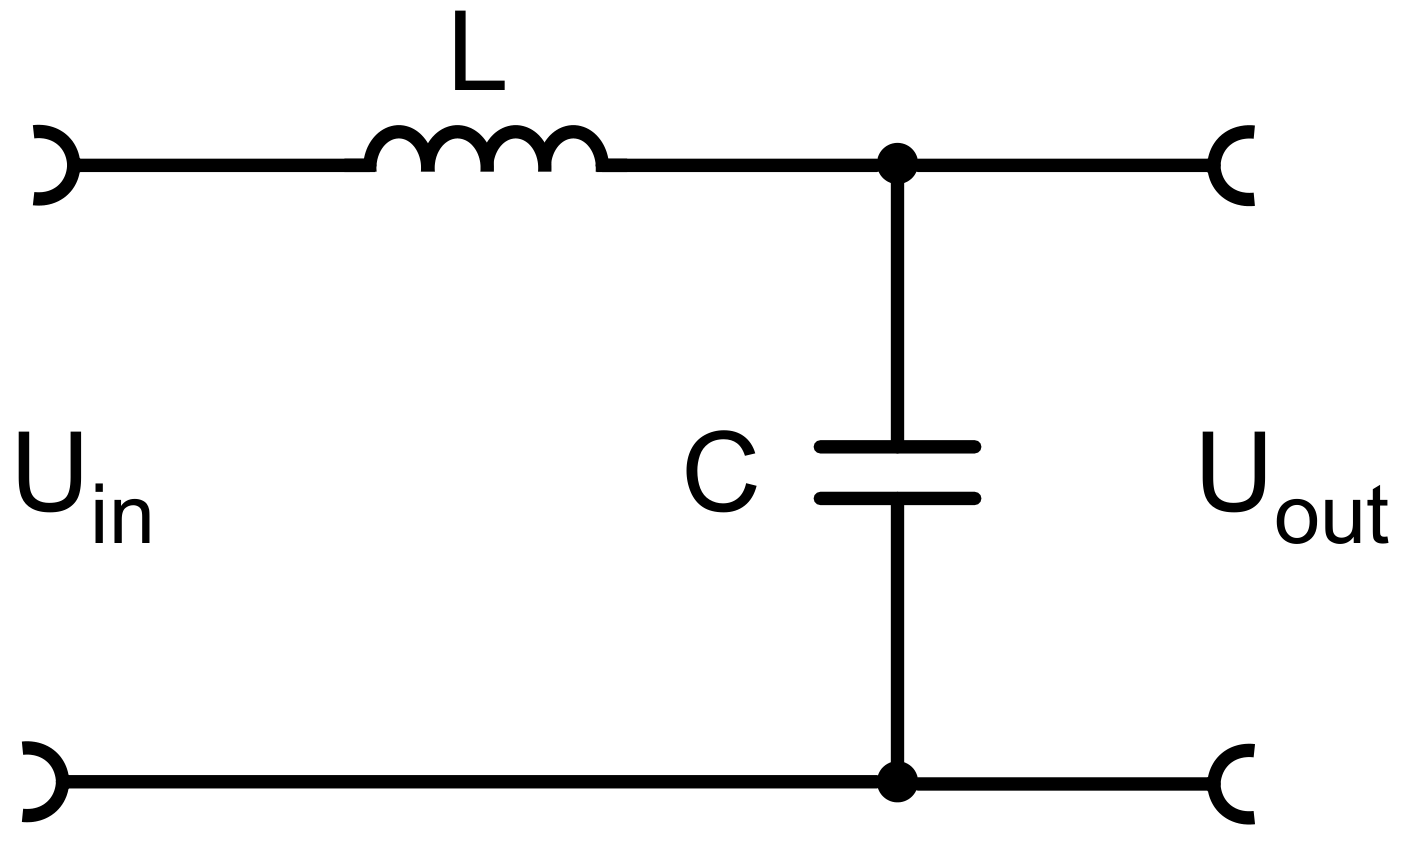
\includegraphics[width=0.3\textwidth]{RC_element}
  \caption{RC-Glied als elementarer Baustein des Koaxkabels}
  \label{fig:rc-element}
\end{figure}

Zur vollständigen mathematischen Beschreibung müssen außerdem Widerstand und Verlustleitwert beachtet werden.
Die Induktivität und Kapazität werden durch die Längsimpedanz $Z \coloneq i\omega L + R$
und Admittanz $Y \coloneq i\omega C + G$, bzw. dementsprechende infinitesimale Größen, ersetzt.
Daraus ergeben sich die DGLs
\begin{align}
  \diff[2]{U}{x} - \Upsilon^2U = 0, \enspace \diff{I}{x} = -U\cdot Y'\\
  \text{mit } \Upsilon^2 = Z'\cdot Y' \nonumber
\end{align}
Die Lösung, mit zusätzlicher Betrachtung der Zeitabhängigkeit, ist für die Spannung
\begin{equation}
  U(x, t) = U_\mr h (x, t) + U_\mr r (x, t) = (U_{\mr h0} e^{-\Upsilon x} + U_{\mr r0} e^{\Upsilon x}) e^{i\omega t} 
\end{equation}
\todo{wo kommt $\omega$ her?}
Es gibt also eine hinlaufende und eine rücklaufende, reflektierte Welle, und die Gesamtspannung entsteht aus Addition dieser Wellen.
Für den Strom ergibt sich eine ähnliche Gleichung, wobei jedoch die rücklaufende Welle einen im Verhältnis zu $U_{\mr r0}$ negativen Beitrag hat.

Das Verhältnis $\frac{U_\mr h}{I_\mr h}$ ist der
\textit{Wellenwiderstand}
\begin{equation}
  Z = \frac{U_\mr h}{I_\mr h} = \sqrt\frac{R' + i\omega L'}{G' + i\omega C'}
\end{equation}
Die Amplitude der rücklaufenden Welle hängt ab vom Abschlusswiderstand
$R_\mr A$, mit dem das Kabelende ($x = l$) belastet wird. Es gilt für den \textit{Reflektionsfaktor} $r = U_{\mr r0} / U_{\mr h0}$
\begin{equation}
  r = \frac{R_\mr A - Z}{R_\mr A + Z}
\end{equation}
Für $R_A = Z$ \question{ist RA dann komplex?} ist also $r = 0$, die gesamte Energie der einlaufenden Welle wird über $R_\mr A$ umgesetzt
und es gibt keine reflektierte Welle. Dieser Zustand wird als \textit{Leitungsanpassung} bezeichnet. Im Leerlauf ($R_\mr A = \infty$)
ist $r=1$ und im Kurzschluss ($R_\mr A = 0$) $r=-1$

Für die Phasen- bzw. Gruppengeschwindigkeit der einlaufenden Welle ergibt sich
\begin{equation}
  v_\mr{ph} = v_\mr{gr} = 1/\sqrt{L'C'} = c_0/\sqrt{\epsilon_r \mu_r}
\end{equation}
also gleicht die Geschwindigkeit der einer Wellenausbreitung im Dielektrikum zwischen den Leitern.



\section{Voraufgaben}
\begingroup
\subsectionAlph

\subsection{}
\subsection{}
\subsection{}

\endgroup

\end{document}
